\documentclass[a4paper,12pt]{article} 

%Добавляет возможность искать и копировать текст
\usepackage{cmap}

%Убирает пробел между названием таблицы/рисунка и самой таблицей/рисунком
\usepackage{caption}
\captionsetup[table]{skip= -0 cm}
\captionsetup[figure]{skip= -0 cm}

%Выравнивание названия таблиц по левому краю
%\usepackage[nooneline]{caption} 
%Размеры отступов 
\usepackage[left=20mm, top=20mm, right=20mm, bottom=20mm, footskip=10mm]{geometry}


%Рисунки
\usepackage{graphicx}
\usepackage{wrapfig} %обтекание элементов
\graphicspath{{graphs}{figures}}  % папки с картинками

%Русский язык в формулах
%\usepackage{mathtext}

%  Русский язык
\usepackage[T2A]{fontenc}			
\usepackage[utf8]{inputenc}			
\usepackage[english,russian]{babel}	

%Готические буквы
\usepackage{amssymb}

% Математика
\usepackage{amsmath,amsfonts,amssymb,amsthm,mathtools} 
\usepackage{wasysym}

%Цветные подписи в таблице
\usepackage[table,xcdraw]{xcolor}

%Красная строка для первого абзаца
\usepackage{indentfirst}

\usepackage{fancyhdr} % Колонтитулы
 	\pagestyle{fancy}
 	\renewcommand{\headrulewidth}{0.3mm}  % Толщина линейки, отчеркивающей верхний колонтитул
 	\lfoot{Белостоцкий А.И}
 	\rfoot{Вовк Д.Е.}
 	\rhead{Кафедра вакуумной электроники}
 	%\chead{Верхний в центре}
 	\lhead{Растровый электронный микроскоп}
 	\renewcommand{\footrulewidth}{0.3mm}
 	\cfoot{\thepage} % По умолчанию здесь номер страницы
 	
\begin{document} 

%Титульник 
\begin{titlepage}
	\begin{center}
		\large 	МИНИСТЕРСТВО ОБРАЗОВАНИЯ И НАУКИ РОССИЙСКОЙ ФЕДЕРАЦИИ\\
				МОСКОВСКИЙ ФИЗИКО-ТЕХНИЧЕСКИЙ ИНСТИТУТ \\
				(НАЦИОНАЛЬНЫЙ ИССЛЕДОВАТЕЛЬСКИЙ ИНСТИТУТ)\\ 
				ФИЗТЕХ-ШКОЛА ЭЛЕКТРОНИКИ, ФОТОНИКИ \\
				И МОЛЕКУЛЯРНОЙ ФИЗИКИ \\
		
		
		\vspace{4.0 cm}
		\LARGE{Кафедра вакуумной электроники \\ 
		Отчет по лабораторной работе} \\ 
		\LARGE \textbf{Растровый электронный микроскоп} \\
	\end{center}
	\vspace{3 cm} \large

	%Надо подумать как это нормально написать	
	\begin{flushleft}
		Работу выполнили \hspace{5.5cm}  \underline{\hspace{3cm}} А.И.Белостоцкий \\	
		\hspace{9.8cm}  \underline{\hspace{3cm}} Д.Е.Вовк \\
		

		\vspace{2cm}
		Работу принял, оценка \hspace{4.5cm} \underline{\hspace{3cm}}
	\end{flushleft}
	
	
	\vfill

	\begin{center}
	Долгопрудный, 2022 г.
	\end{center}
\end{titlepage}                                                                      

\tableofcontents

\newpage

\section{Аннотация}

Во многих областях физики твердого тела, а также в геологии,
металлургии, биофизике нередко возникает потребность исследовать
элементный состав какого-либо образца не только в целом, но и узнать
локальное распределение различных химических элементов на его
поверхности. Такую возможность предоставляет электронно-зондовый
микроанализатор – растровый микроскоп, позволяющий «видеть», из
каких атомов состоит поверхность изучаемого образца. Почти любой
современный растровый (или реже просвечивающей) электронный
микроскоп оснащен приставкой, позволяющими измерять рентгеновские
спектры. Принцип растровой электронной микроскопии (РЭМ) состоит в
сканировании исследуемой поверхности тонким электронным лучом по
типу телевизионной развёртки. Выбитые электронным лучом вторичные
электроны или рентгеновские кванты регистрируются детектором
электронов. Интенсивность полученного с детектора сигнала определяет
яркость точки растра на итоговом изображении. 

Данная лабораторная работа направлена на ознакомление студентов с
физическими принципами функционирования РЭМ и одной из методик –
электронно-зондового микроанализа. Экспериментальная часть работы
заключается в ознакомлении с принципом действия растрового
электронного микроскопа JOEL JSM-7001F, а также в применении
рентгеновского микроанализа для определения элементного состава
образцов.

\section{Экспериментальная установка}

Микроскоп, изучаемый в ходе данной работы, позволяет вести
наблюдения образца в трех основных режимах: во вторичных электронах,
в отраженных электронах, в рентгеновских лучах (микроанализатор). Для
первых двух режимов оптимальный ток с точки зрения точности
результатов составляет 1-1000 пА, при рентгеновском микроанализе
оптимальным считается ток зонда порядка 100 нА. Поэтому ток зонда
микроскопа изменяется в широких пределах.

Структурная схема микроскопа дана на рис. \ref{setup} Рассмотрим все по
порядку, начиная с формирования электронного зонда. Ускорение и
фокусировка пучка происходит в колонне, вверху которой находится
электронная пушка, испускающая электроны. Далее следует система
электронной оптики, которая формирует узкий зонд, а также позволяет
отклонять его в сторону, направляя в определенные точки образца. Во внутренних областях колонны поддерживается вакуум, чтобы избежать
рассеяния электронов и окисления вольфрамовой нити, являющейся
источником электронов.

Образец крепится в специальном держателе, позволяющем
максимально удобно оперировать с образцами в процессе работы.
Образец окружен детектирующей аппаратурой — детектором отражённых электронов, детектором вторичных электронов, рентгеновским спектрометром.

\begin{figure}[h]
    \centering
    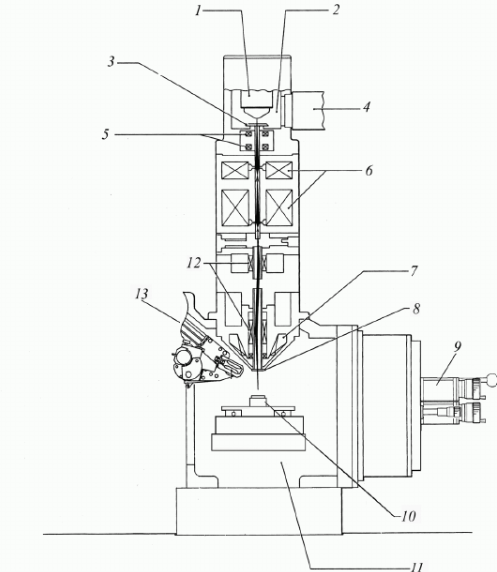
\includegraphics[width = 0.5\linewidth]{fig3.png}
    \caption{Общая схема растрового электронного микроскопа:
1 — электронная пушка; 2 — камера электронной пушки;
3 — анод; 4 — вакуумная магистраль; 5 — юстировочные катушки;
6 — конденсорные линзы; 7 — объектная линза; 8 — детектор упругоотражённых
электронов; 9 — система позиционирования образцов; 10 — держатель образцов; 11 — основная вакуумная камера; 12 — сканирующие катушки; 13 — рентгеновский спектрометр}
    \label{setup}
\end{figure}
 
 \newpage
 
\section{Ход работы}

\subsection{Каналирование}

Разработка специальных экспериментальных методик (анализ картин дифракции обратнорассеянных электронов) сделала возможным проводить структурных анализ поликристаллических материалов с разрешением порядка 1 мкм. В кристаллическом твердом теле периодичность расположения атомов может оказывать влияние на то, как происходит взаимодействие первичных электронов, в особенности на начальном этапе взаимодействия вблизи поверхности. В частности рассмотрим эффект каналирования электронов, который возникает из-за различия в плотности упаковки атомов вдоль различных кристаллографических направлений. Для первичных электронов с ростом глубины от поверхности вероятность выхода из твердого тела уменьшается почти экспоненциально.Таким образом, те электроны, которые первично проникли в кристал вдоль <<каналов>>, имеют более низкую вероятность выхода из кристалла, чем те электроны, которые провзаимодействовали в первом слое атомов. 

Для описания свойств высокоэнергетических первичных электронов внутри кристалла можно использовать модель блоховских волн. При взаимодействии с группой кристаллических плоскостей, расстояние между которыми -- d,  соотношение между <<проходящими>> и <<застревающими>> волнами одинаково при выполнении условия Брэгга-Вульфа:

\[
    n \lambda = 2d \sin \theta, n \in \mathbb{Z_+}
\]

На практике, данное условие означает, что мы будем получать изображение с темными участакми (все электроны <<прошли>>) и светлыми (все электроны отразились).

Получим избражение образцов монокристаллов кремния с разной ориентаций.

\begin{figure}[h]
\centering
\begin{minipage}{.5\textwidth}
  \centering
  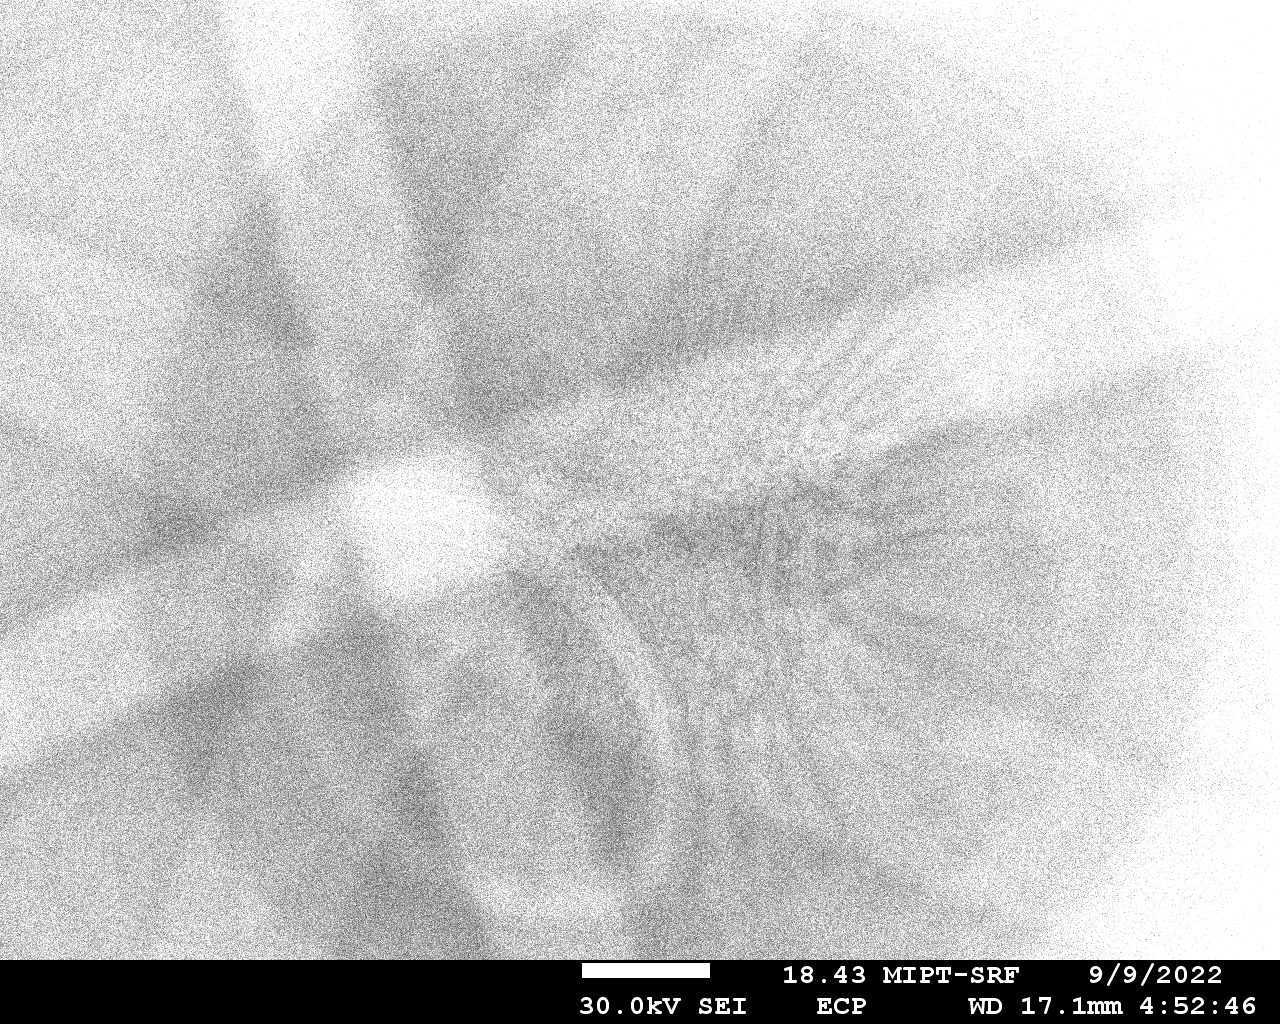
\includegraphics[width=1\linewidth]{Si006 (1).jpg}
  \captionof{figure}{Первый образец кремния}
  \label{fig:Si006}
\end{minipage}%
\begin{minipage}{.5\textwidth}
  \centering
  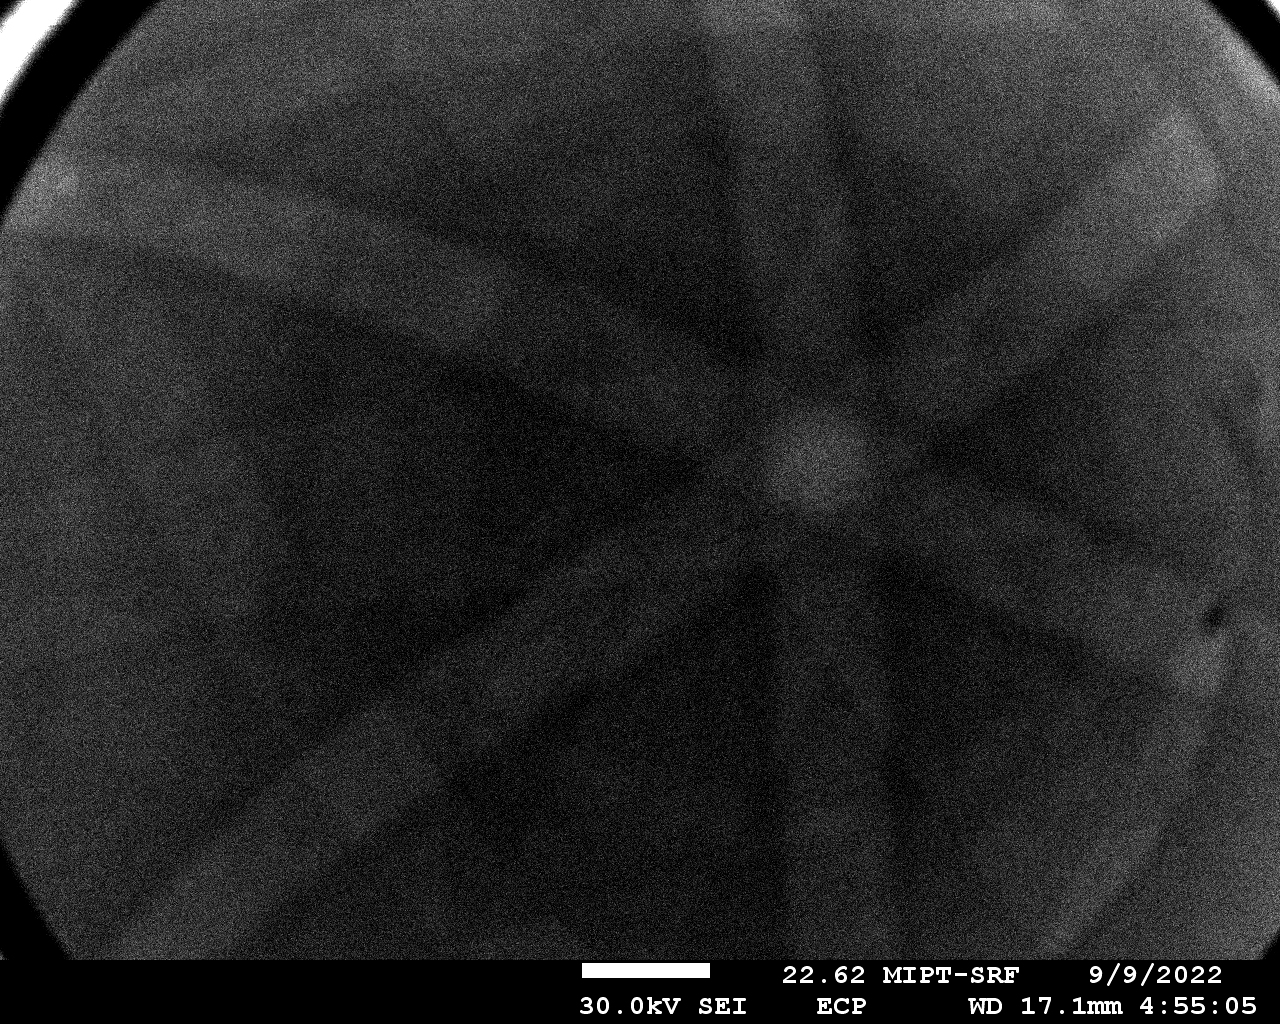
\includegraphics[width=1\linewidth]{Si007.jpg}
  \captionof{figure}{Второй образец кремния}
  \label{fig:Si007}
\end{minipage}
\end{figure}

Таким образом, мы получили картины каналирования в образцах кремния с различной ориентацией и убедились в том, что он, действительно, является монокристаллом.


\subsection{Топографический и материальный контрасты. Спектроскопия}
\begin{wrapfigure}{r}{0.3\textwidth} 
    
    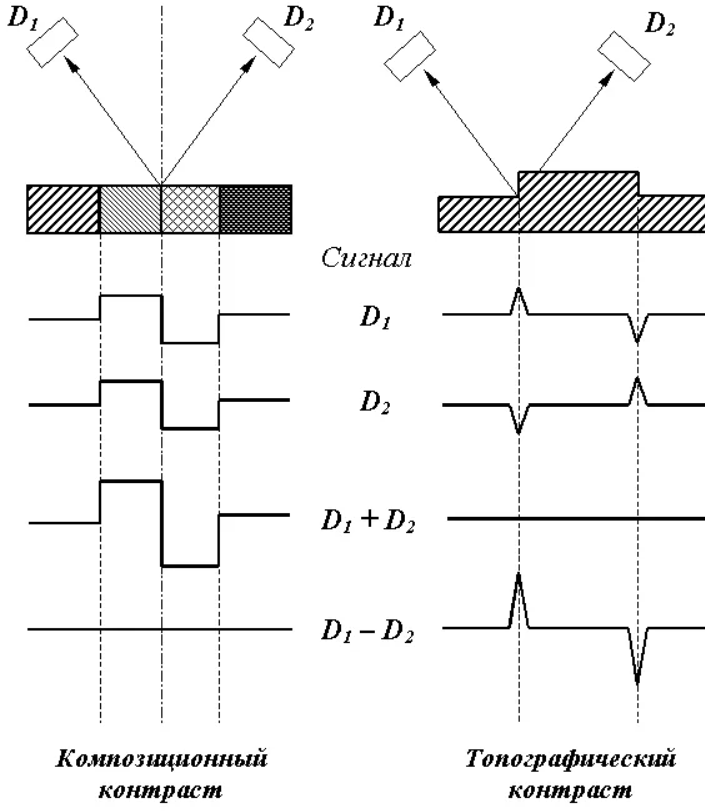
\includegraphics[width=0.30\textwidth]{контраст.png}
    \caption{схема получения контрастов}
    \label{contr}
\end{wrapfigure}
Детектор вториччных электронов представляет собой две отдельные  полукруглые секции. Рассматривая сумму или разность сигналов с этих половинок можно можно наблюдать топографический или композиционный контрасты (\ref{contr}).

В режиме топографического контраста отраженные значение выводимой разницы сигналов сильно зависит от формы поверхности. Поэтому на фотографии \ref{fig:topograph}, сделанной в этом режиме мы видим рельеф местности. В режиме суммы не играет роли то, в каком направлении летели попавшые на детектор электроны. Поэтому рельеф на фотографии \ref{fig:komp} не виден. Однако количество электронов напрямую зависит от номера элемента. И пятна обозначают собой границы различных компонент таблетки. На этом этапе можно уже сделать вывод, что таблетка сделана из двух несмешиваемых металлов (второе можно предположить по металлическому цвету).


В итоге мы получили информацию о рельефе поверхности и установили тот факт, что таблетка состоит из 2х различных материалов, а также их распределение. Однако мы все еще не можем сделать вывод о том, какие именно это элементы. В этом на поможет аналих рентгеновского излучения. Так как каждый элемент излучает на своих частотах.

\newpage

\begin{figure}[h]
\centering
\begin{minipage}{.5\textwidth}
  \centering
  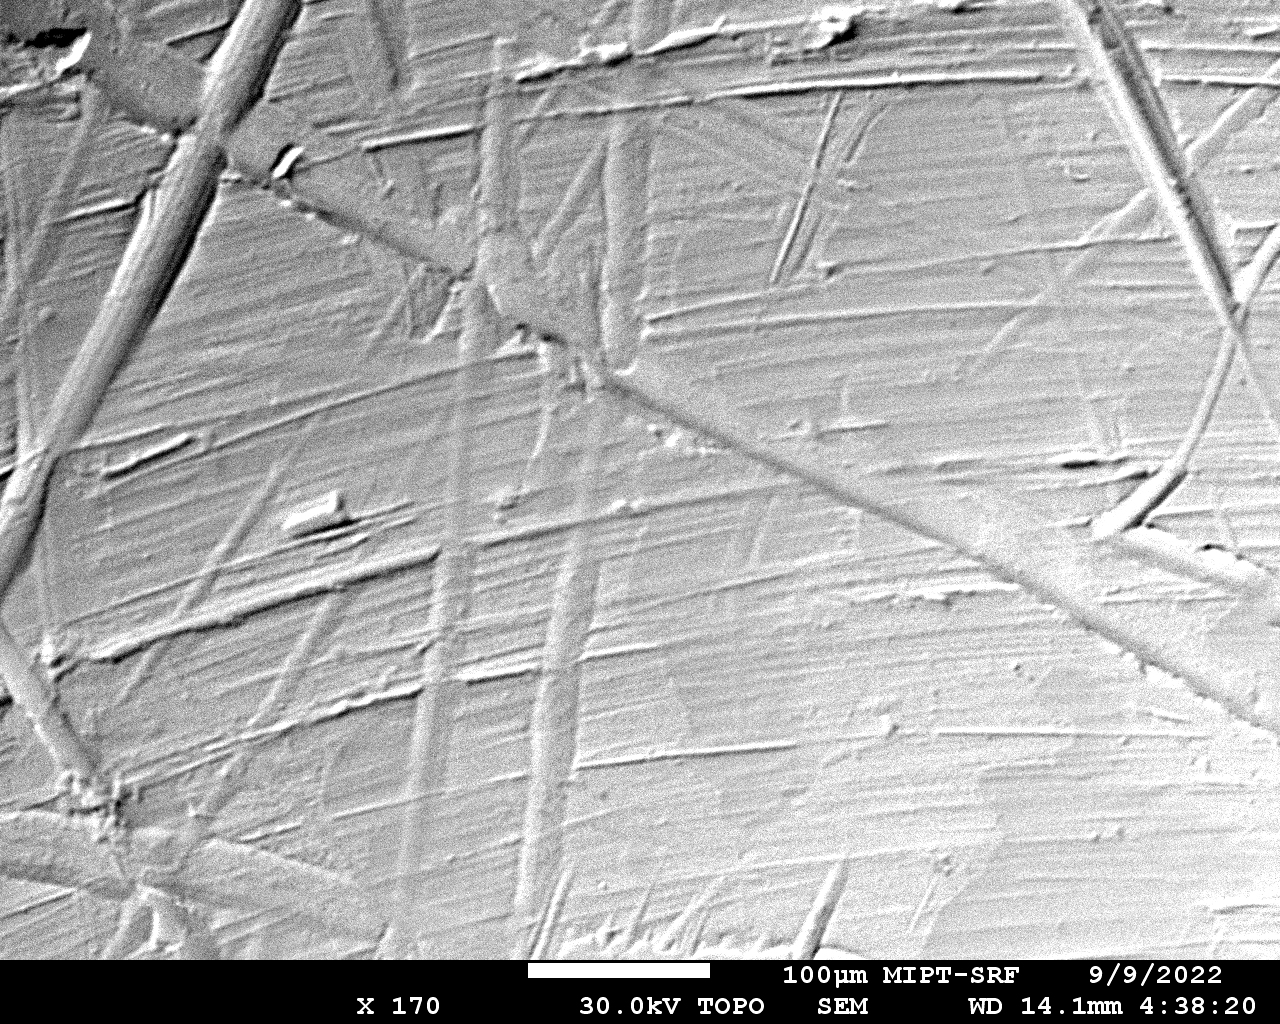
\includegraphics[width=1.2\linewidth]{Tablet005.jpg}
  \captionof{figure}{Топографический контраст}
  \label{fig:topograph}
\end{minipage}%
\begin{minipage}{.5\textwidth}
  \centering
  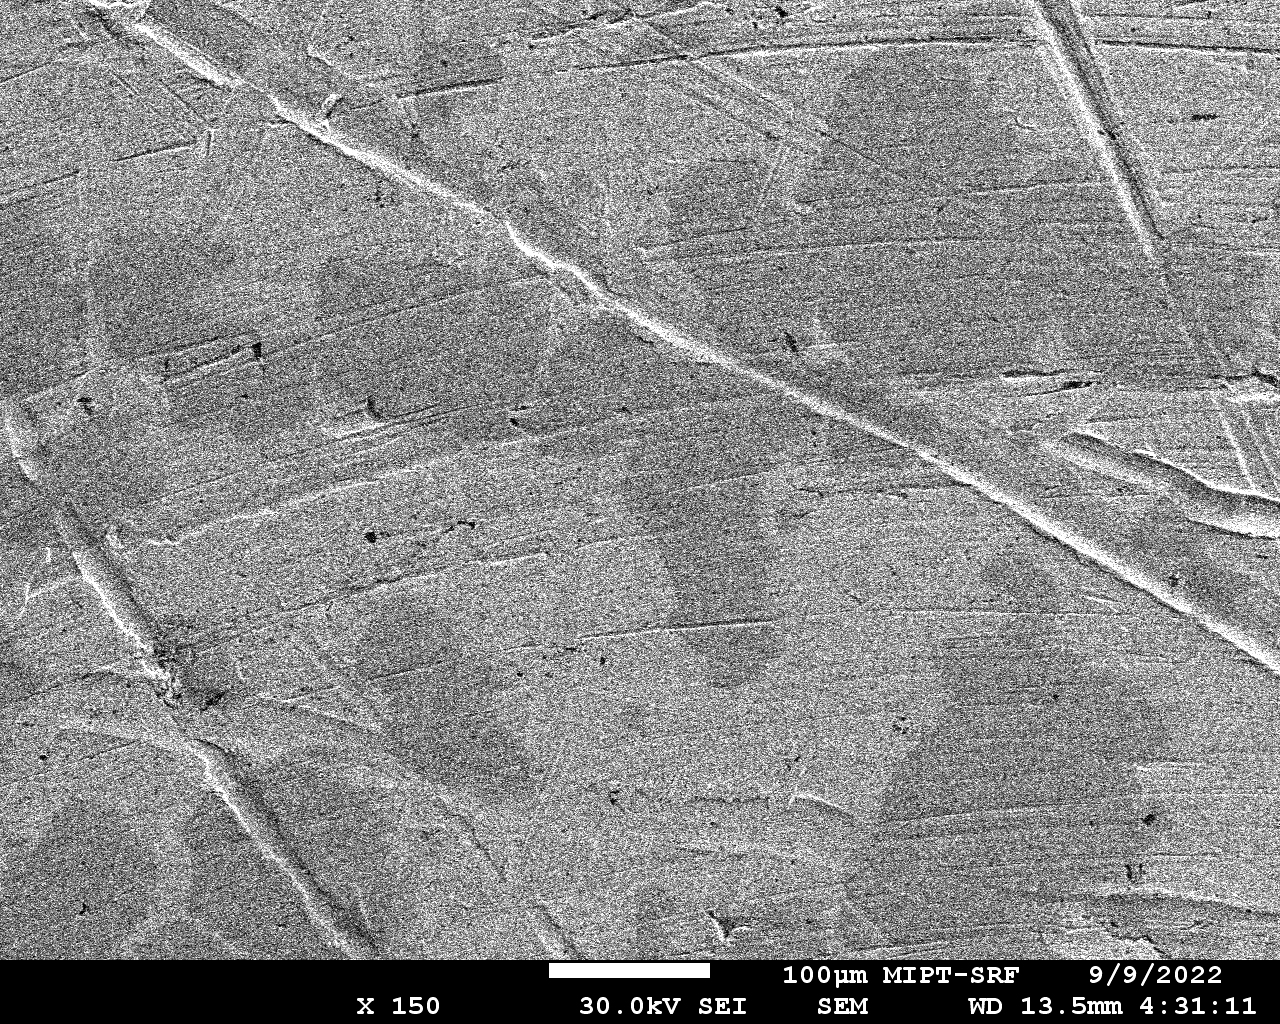
\includegraphics[width=1.2\linewidth]{Tablet001.jpg}
  \captionof{figure}{Композиционный контраст}
  \label{fig:komp}
\end{minipage}
\end{figure}

С помощью анализатора энергии фотонов. Мы можем получить спектр излучения таблетки \ref{fig:spectra}.  Теперь мы видим, что металлы, из которых сделана таблетка - это хром и медь. Минусом этого метода является то, что получить информацию таким образом мы модежем только о составе поверхности образца из-за низкой толщины зоны, откуда могут выйти фотоны.

\begin{figure}[h]
    \centering
    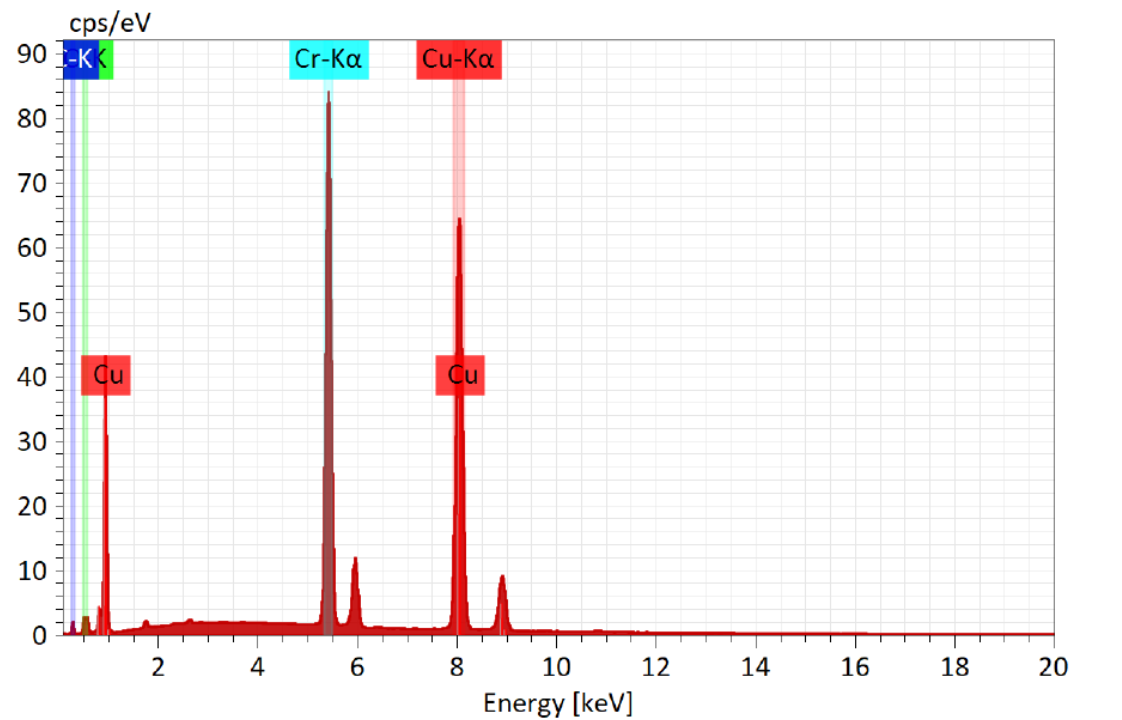
\includegraphics[width=0.9\linewidth]{Spectra.png}
    \caption{Спектр излучения таблетки}
    \label{fig:spectra}
\end{figure}
 Мы также видим наличие некоторое количество ядер O С.
 Мы можем посмотреть на распредление количества этих элементов относительно цинка и меди. Для этого сначала посмотрим на их расположение (\ref{fig:Cu} и \ref{fig:Cr}).
 
 \begin{figure}[h]
\centering
\begin{minipage}{.5\textwidth}
  \centering
  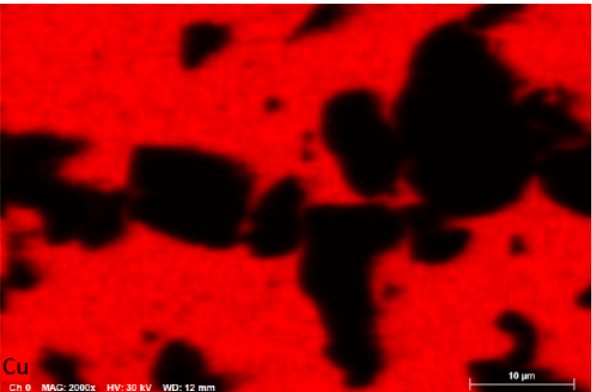
\includegraphics[width=1\linewidth]{Cu.png}
  \captionof{figure}{Медь}
  \label{fig:Cu}
\end{minipage}%
\begin{minipage}{.5\textwidth}
  \centering
  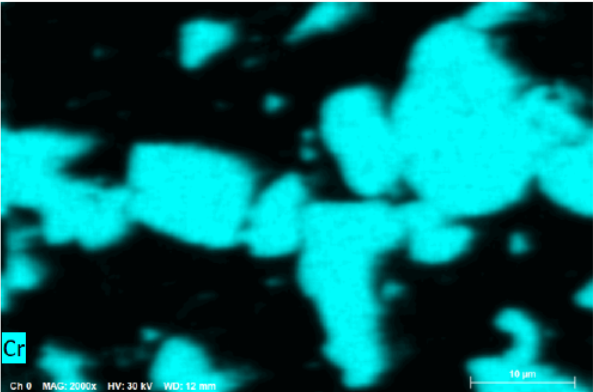
\includegraphics[width=1\linewidth]{Cr.png}
  \captionof{figure}{Хром}
  \label{fig:Cr}
\end{minipage}
\end{figure}
 
 А теперь на C и O (\ref{fig:C} и \ref{fig:O}).
 \begin{figure}[h]
\centering
\begin{minipage}{.5\textwidth}
  \centering
  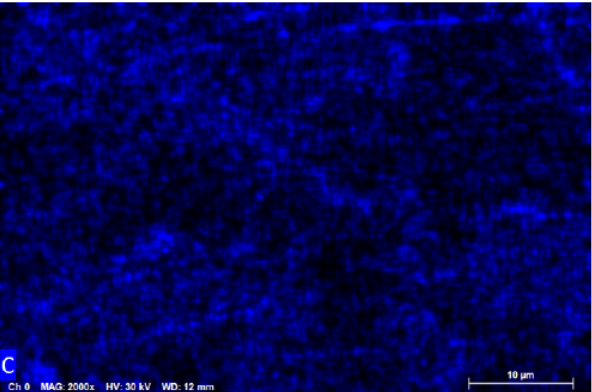
\includegraphics[width=1\linewidth]{C.png}
  \captionof{figure}{Углерод}
  \label{fig:C}
\end{minipage}%
\begin{minipage}{.5\textwidth}
  \centering
  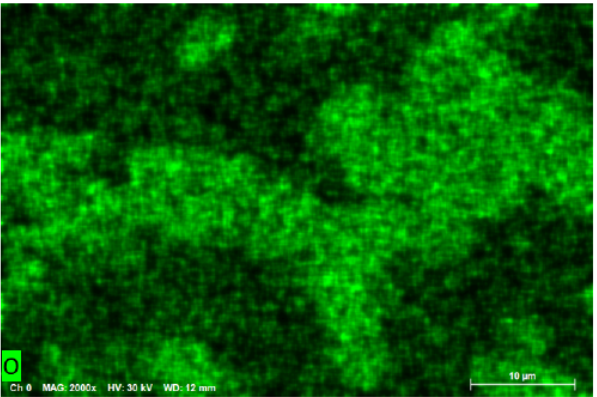
\includegraphics[width=1\linewidth]{O.png}
  \captionof{figure}{Кислород}
  \label{fig:O}
\end{minipage}
\end{figure}
Методом пристального взгляда видно, что ислорода больше в областях хрома, а углерода, наоборот, на меди. Это может быть связано с тем, что Хром бывает трех и 6ти валентный, те существуют оксиды Cr2O3 и CrO3, хотя второй и нестабильный. В то время как оксид меди бывает только CuO. И кислорода в оксидной пленке на поверхности просто больше у хрома.


\textbf{Интересные наблюдения}
С помощью РЭМ можно рассмотреть структуру крыла мотылька: чешуйки и дифракцинную решетку, из-за которой крылья могут иметь различные яркие раскраски.
\begin{figure}[h!]
\centering
\begin{minipage}{.5\textwidth}
  \centering
  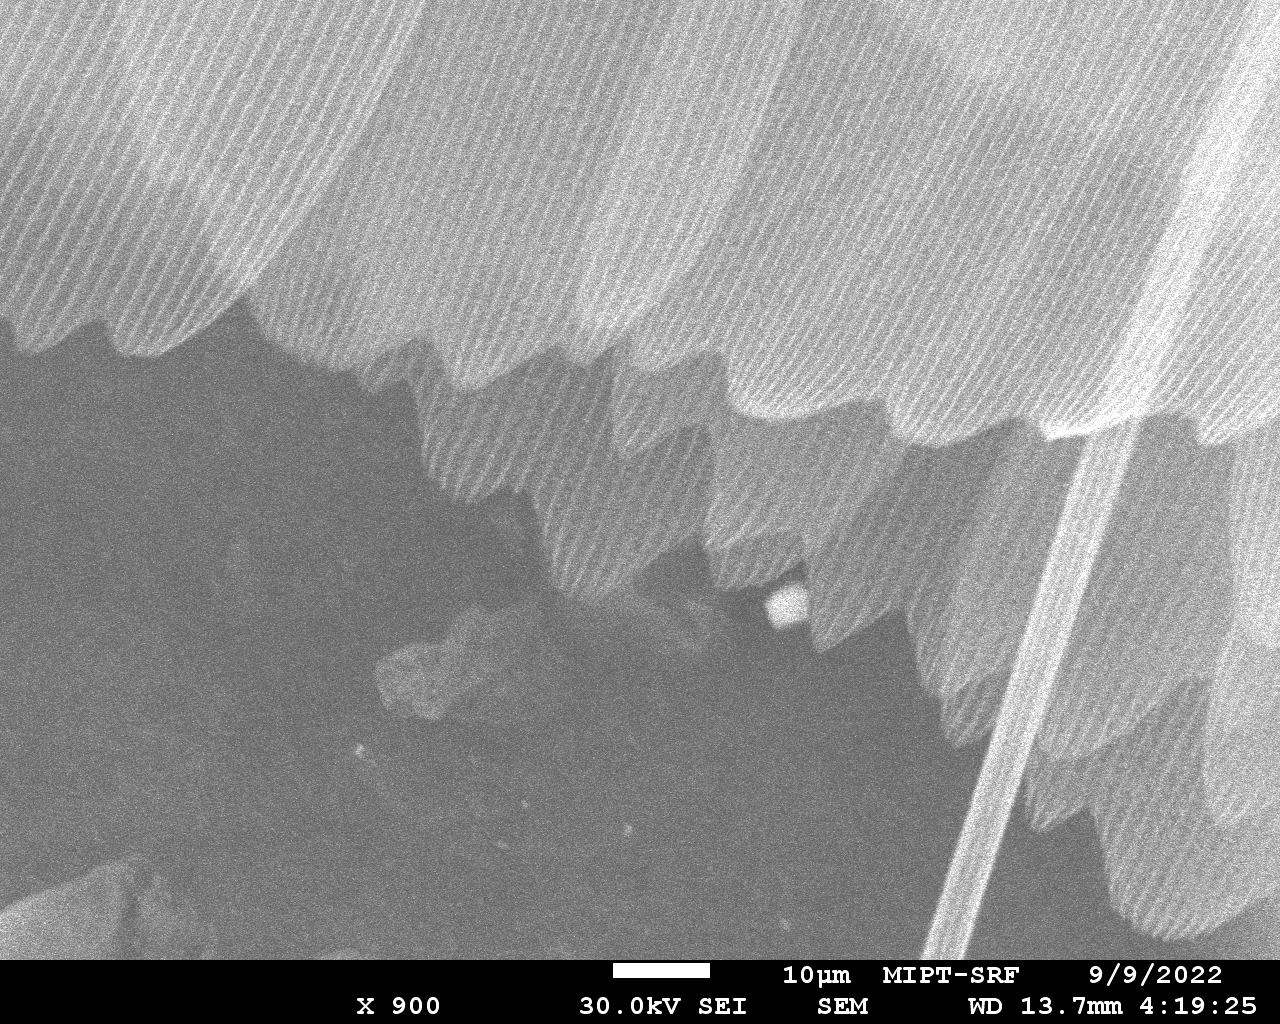
\includegraphics[width=1\linewidth]{Butterfly001.jpg}
  
\end{minipage}%
\begin{minipage}{.5\textwidth}
  \centering
  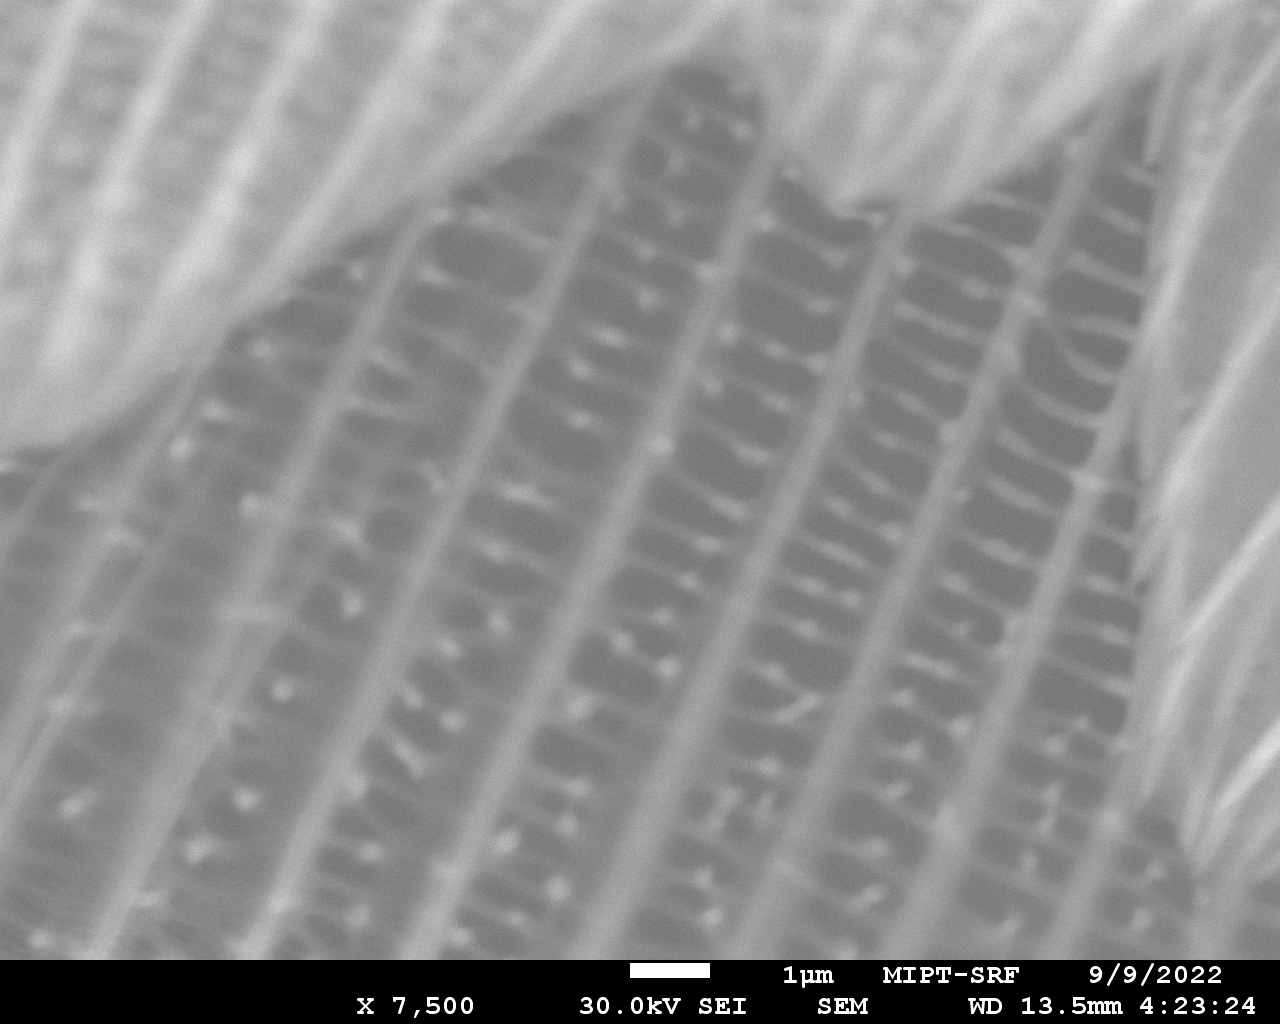
\includegraphics[width=1\linewidth]{Butterfly003.jpg}
  
\end{minipage}
\end{figure}

\subsection{Получение изображения внутренней камеры микроскопа}

Поместим в микроскоп диэлектрическим образец (пенопласт). В силу того, что для диэлектриков $\eta$ < 1 (коэффииент неупругого отражения) образец начнет приобретать отрицательный заряд. Тогда, установив небольшую энергию для электронов, через какое-то время они перестанут долетать до образца, так как им не будет хватать энергии, следовательно они будут выбивать вторичные электроны из внутренней поверхности микроскопа. Таким образом, можно получить изображение вакуумной части микроскопа. Данные изображения представлены на рисунках \ref{fig:Inside1} и \ref{fig:Inside2}





\begin{figure}[h!]
\centering
\begin{minipage}{.5\textwidth}
  \centering
  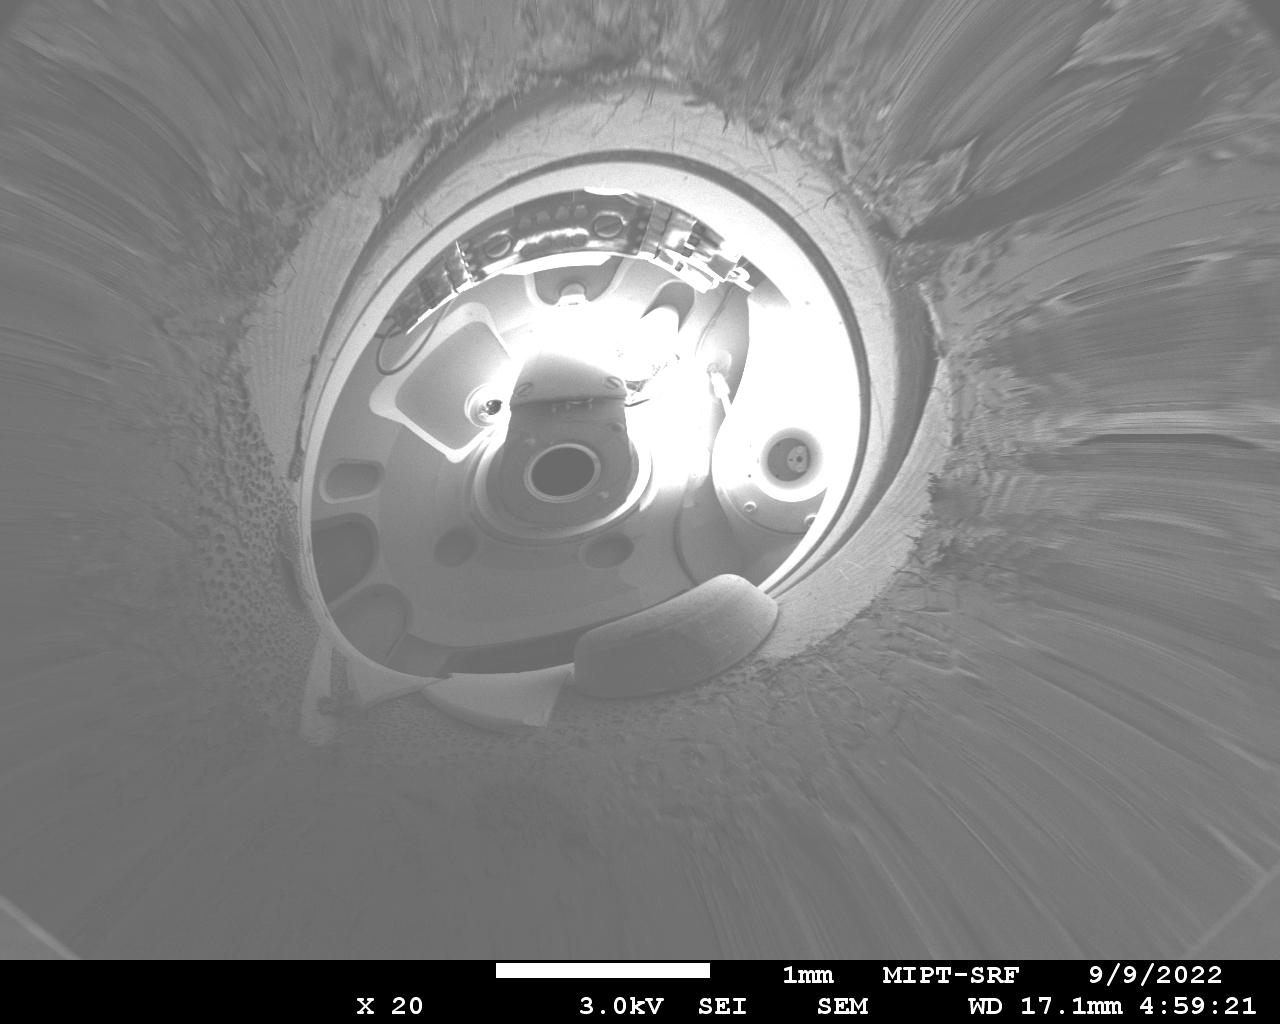
\includegraphics[width=1\linewidth]{Foam009.jpg}
  \captionof{figure}{Изображения внутренней \\ камеры микроскопа}
  \label{fig:Inside1}
\end{minipage}%
\begin{minipage}{.5\textwidth}
  \centering
  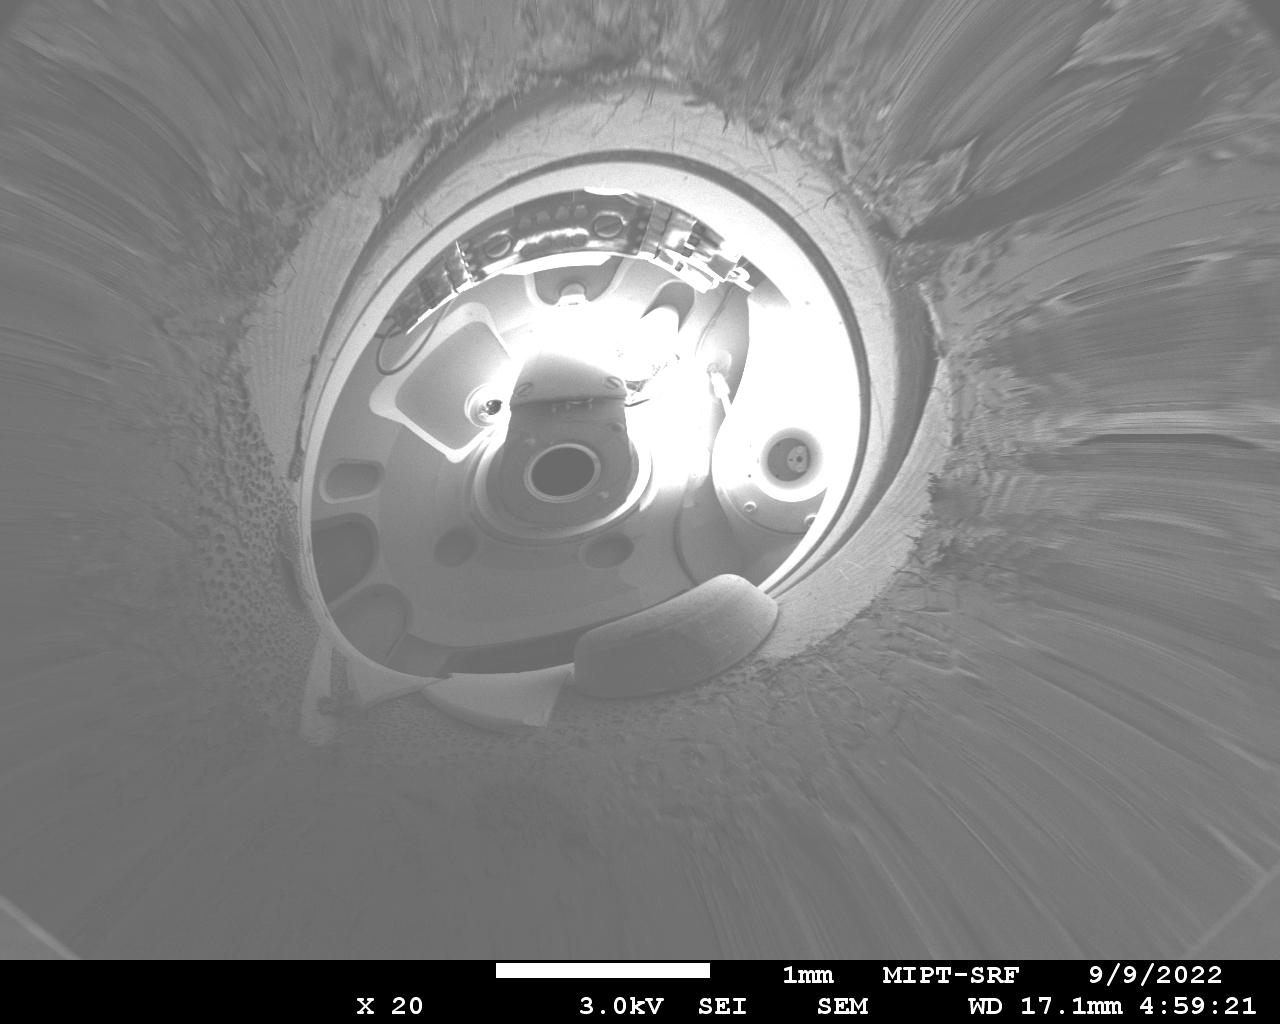
\includegraphics[width=1\linewidth]{Foam009.jpg}
  \captionof{figure}{Изображения внутренней \\ камеры микроскопа}
  \label{fig:Inside2}
\end{minipage}
\end{figure}

\section{Выводы}
Таким образом, мы освоили базовые физические принципы функционирования РЭМ и основные методики измерения.В том числе:

\begin{itemize}
    \item Получили изображение образца в различных режимах работы микроскопа (SE и BSE)
    \item Изучили физические принципы формирования изображения в РЭМ
    \item Применили рентгеновский микроанализ для определения элементного состава образца
    \item Получили картины каналирования в образцах монокристаллического кремния с различной ориентацией
\end{itemize}








\end{document}
